% Line Atlas chapter draft.
% Suggested dependencies: amsmath, amssymb, siunitx, booktabs, tabularx,
% tikz, pgfplots, xcolor, hyperref.

\chapter{Star Formation Across Scales and the Lines That Trace It}
\label{chap:star-formation}
\chaptermark{Star Formation and Its Tracers}

Star formation connects parsec-scale self-gravitating structures to the integrated
light of galaxies.  Spectral lines enter at every stage: molecular transitions map
the reservoir, dense-gas species select compact structures, infall and outflow shape
profiles, recombination lines count ionizing photons, and metal lines diagnose the
H\,II regions around massive stars.  No single transition measures an instantaneous,
scale-independent ``star-formation rate.''  Each tracer averages over a population,
timescale, extinction geometry, and aperture.

This chapter builds a hierarchy from collapse physics to population calibrations.
Broad theoretical and observational syntheses are provided by
\citet{McKeeOstriker2007} and \citet{KennicuttEvans2012}; dense-core physics is
reviewed by \citet{BerginTafalla2007}.

\section{Gravity, pressure, and characteristic scales}

For isothermal gas of density $\rho$ and sound speed $c_s$, the Jeans length and a
commonly used Jeans mass convention are
\begin{equation}
 \lambda_J=c_s\left(\frac{\pi}{G\rho}\right)^{1/2},
 \qquad
 M_J=\frac{\pi^{5/2}}{6}\frac{c_s^3}{G^{3/2}\rho^{1/2}}.
 \label{eq:jeans-scales}
\end{equation}
Perturbations larger than the Jeans length can grow in the idealized infinite,
uniform, nonmagnetic medium.  Real clouds are finite, turbulent, magnetized, and
externally pressured; Jeans quantities remain useful local scales rather than exact
fragmentation predictions.

The free-fall time of a uniform sphere is
\begin{equation}
 t_{\rm ff}=\left(\frac{3\pi}{32G\rho}\right)^{1/2}.
 \label{eq:free-fall-time}
\end{equation}
Star formation is inefficient per mean-density free-fall time.  A common descriptive
parameter is
\begin{equation}
 \epsilon_{\rm ff}=\frac{\dot M_\star t_{\rm ff}}{M_{\rm gas}}.
 \label{eq:epsilon-ff}
\end{equation}
Its inferred value depends on how a cloud boundary, gas mass, density, stellar
population, and averaging time are defined.  A region that is assembling or
dispersing violates the steady-state interpretation of $\dot M_\star$.

Thermal pressure is rarely the dominant cloud-scale support.  A useful effective
one-dimensional dispersion may combine thermal and nonthermal motions,
\begin{equation}
 \sigma_{\rm eff}^2=c_s^2+\sigma_{\rm nt}^2,
 \label{eq:effective-dispersion}
\end{equation}
but calling every nonthermal line width ``support'' is dangerous.  Converging flows,
rotation, collapse, opacity broadening, and unresolved components all contribute.
Support is a statement about the momentum equation and spatial correlations, not
about linewidth alone.

\subsection{Worked example: free-fall time of a dense clump}

Take molecular gas with number density
$n_{\rm H_2}=10^4\,\mathrm{cm^{-3}}$ and mean mass per H$_2$ molecule including helium
$\mu_{\rm H_2}m_{\rm H}\simeq2.8m_{\rm H}$.  Then
$\rho\simeq4.7\times10^{-20}\,\mathrm{g\,cm^{-3}}$ and
\begin{equation}
 t_{\rm ff}\simeq3.1\times10^5~\mathrm{yr}.
\end{equation}
If the clump has $M=10^4M_\odot$ and
$\epsilon_{\rm ff}=0.01$, its time-averaged star-formation rate would be
$\dot M_\star\simeq3.2\times10^{-4}M_\odot\,\mathrm{yr^{-1}}$.  This estimate is
conditional on the mean density and on a steady efficiency; substructure has shorter
local free-fall times.

\section{Magnetic fields and mass-to-flux balance}

Magnetic fields affect compression, angular-momentum transport, anisotropic motion,
and the coupling of protostellar outflows to gas.  A cloud's mass-to-flux ratio is
often compared with a critical value,
\begin{equation}
 \mu_\Phi\equiv\frac{(M/\Phi_B)}{(M/\Phi_B)_{\rm crit}}.
 \label{eq:mass-to-flux}
\end{equation}
Subcritical structures ($\mu_\Phi<1$) cannot collapse across ordered field lines in
ideal magnetohydrodynamics, while supercritical structures can.  The numerical
critical coefficient depends on geometry.  Zeeman splitting measures a line-of-sight
field component in selected gas, dust polarization traces projected orientation with
grain-alignment assumptions, and Faraday rotation weights $n_eB_\parallel$.  Combining
these into a three-dimensional field demands a geometric model.

Nonideal effects---ambipolar diffusion, Ohmic dissipation, and the Hall effect---allow
field and neutral matter to drift on small scales.  Turbulent reconnection and field
topology further complicate a single diffusion-time picture.  Magnetic criticality
should therefore be inferred as a distribution with projection uncertainty, not a
binary label for one projected map.

\section{From clouds to filaments, clumps, and cores}

Cloud structure is scale free over substantial ranges, and names such as clump and
core partly reflect resolution and tracer choice.  A dense continuum peak may contain
several velocity components; a velocity-coherent feature may have little contrast in
column density.  Catalog completeness depends on spatial filtering and segmentation.

Dense cores are often categorized as starless, prestellar, or protostellar.  A
prestellar designation implies gravitational boundedness, which inherits uncertainty
from mass, temperature, radius, linewidth, density profile, magnetic field, and
external pressure.  A source without an infrared counterpart is not automatically
starless: deeply embedded low-luminosity objects can evade a survey.

Chemical differentiation provides an evolutionary clock only after physical
conditions are modeled.  CO freeze-out at cold high density can enhance N$_2$H$^+$
relative to CO; protostellar heating returns volatile species to the gas; shocks
release grain material and enhance molecules such as SiO.  Reaction and adsorption
timescales vary with density, temperature, ionization, and grain surface area.  A
chemical ``age'' is model dependent.

\section{Infall and accretion signatures}

An optically thick line with an excitation temperature rising inward can show a
brighter blue peak than red peak when the envelope is collapsing and a thinner line
defines the systemic velocity.  The foreground redshifted layer preferentially
absorbs red emission.  This classic blue asymmetry is suggestive, not unique:
multiple clouds, rotation, outflow, and spatially varying excitation can mimic it.
Mapping and comparison of optically thick and thin isotopologues are essential.

Mass infall is sometimes estimated as
\begin{equation}
 \dot M_{\rm inf}=4\pi r^2\rho(r)v_{\rm inf}(r).
 \label{eq:mass-infall-rate}
\end{equation}
Every factor is model dependent.  A fitted profile constrains projected velocity
through a radiative-transfer model; it does not directly measure a spherical mass
flux.  Filamentary accretion, disks, and episodic flow can make the spherical estimate
an orientation-level summary only.

Accretion luminosity onto a protostar of mass $M_\star$ and radius $R_\star$ is
approximately
\begin{equation}
 L_{\rm acc}\simeq f_{\rm acc}\frac{GM_\star\dot M_{\rm acc}}{R_\star},
 \label{eq:accretion-luminosity}
\end{equation}
where $f_{\rm acc}$ accounts for energy advected, radiated elsewhere, or carried by
outflows.  Hydrogen lines such as Br$\gamma$ may correlate empirically with accretion
luminosity in calibrated samples, but geometry, extinction, winds, and stellar mass
limit extrapolation.

\section{Protostellar jets and molecular outflows}

Magnetocentrifugal launching extracts angular momentum and produces fast jets or
winds.  Their interaction entrains molecular gas into broad line wings.  CO maps can
estimate outflow mass, momentum, and kinetic energy after corrections for excitation,
opacity, missing low-velocity gas, abundance, spatial filtering, and inclination.
For channel mass $M(v)$ relative to systemic velocity,
\begin{align}
 P_{\rm out}&=\sum_v M(v)|v-v_{\rm sys}|,\\
 E_{\rm out}&=\frac{1}{2}\sum_vM(v)(v-v_{\rm sys})^2.
 \label{eq:outflow-momentum-energy}
\end{align}
Energy is especially sensitive to faint high-velocity wings, while mass is sensitive
to confusion near the cloud velocity.  A dynamical time $t_{\rm dyn}=R_{\rm proj}/
v_{\rm los}$ combines two projection-dependent quantities and is not necessarily the
true age.  Reporting uncorrected observables alongside model-corrected rates helps
future reinterpretation.

Shock-excited H$_2$, [Fe\,II], SiO, and high-$J$ CO trace different zones of an
outflow.  [Fe\,II] can indicate fast, partially ionized shocks and grain processing;
near-infrared H$_2$ lines select warm molecular material; low-$J$ CO carries much of
the cool entrained mass.  Line luminosity alone cannot inventory the outflow without
a temperature distribution.

\section{\texorpdfstring{H\,II}{H II} regions as ionizing-photon calorimeters}

For uniform hydrogen density $n_{\rm H}$ around a source emitting $Q_{\rm H}$ ionizing
photons per second, the ideal Str\"omgren radius is
\begin{equation}
 R_S=\left(\frac{3Q_{\rm H}}{4\pi\alpha_Bn_e n_p}\right)^{1/3}.
 \label{eq:stromgren-radius}
\end{equation}
After rapid ionization, overpressure drives expansion.  An idealized uniform-medium
solution is
\begin{equation}
 R(t)=R_S\left(1+\frac{7c_it}{4R_S}\right)^{4/7},
 \label{eq:hii-spitzer-expansion}
\end{equation}
where $c_i$ is ionized-gas sound speed.  Density gradients, winds, radiation pressure,
leakage, gravity, magnetic fields, and cloud porosity change the evolution.

The observed recombination luminosity counts ionizations absorbed by gas.  If a
fraction $f_{\rm esc}$ escapes and $f_{\rm dust}$ is absorbed by dust before ionizing
hydrogen, then schematically
\begin{equation}
 Q_{\rm H,gas}=(1-f_{\rm esc}-f_{\rm dust})Q_{\rm H,total}.
 \label{eq:ionizing-photon-budget}
\end{equation}
Age and IMF determine $Q_{\rm H,total}$ per unit star-formation rate.  Binary evolution
and stellar rotation can extend hard ionizing emission beyond the lifetime predicted
by a simple single-star population.

\subsection{Worked example: Str\"omgren scale}

For $Q_{\rm H}=10^{49}\,\mathrm{s^{-1}}$, $n_e\simeq n_p=100\,\mathrm{cm^{-3}}$,
and $\alpha_B=2.6\times10^{-13}\,\mathrm{cm^3\,s^{-1}}$,
\begin{equation}
 R_S\simeq3.1~\mathrm{pc}.
\end{equation}
Reducing density by a factor of ten increases $R_S$ by $10^{2/3}\simeq4.6$.
The calculation assumes uniform fully ionized hydrogen and no dust or leakage; a
clumpy nebula with the same mean density need not have the same recombination rate.

\section{Star-formation-rate tracers as temporal filters}

A luminosity-based calibration can be written
\begin{equation}
 \dot M_\star=C_XL_X,
 \label{eq:sfr-calibration-generic}
\end{equation}
but $C_X$ encodes an IMF, metallicity, stellar-evolution model, star-formation history,
dust treatment, and luminosity definition.  More fundamentally, the luminosity is a
convolution of the past star-formation history with a response kernel,
\begin{equation}
 L_X(t)=\int_0^\infty \dot M_\star(t-\tau)\,
 \ell_X(\tau,Z,\mathrm{IMF})\,\mathrm{d}\tau.
 \label{eq:sfr-response-kernel}
\end{equation}
Ionizing-recombination tracers weight the youngest massive stars; ultraviolet
continuum persists longer; supernova-related radio emission is delayed; infrared
emission depends on dust heating and can include older stars.  Differences among
tracers may reveal burstiness rather than calibration failure.

\begin{table}[tbp]
\centering
\caption{Common star-formation tracers and dominant qualifications.  Timescales are
population dependent and should be computed for the adopted stellar model.}
\label{tab:sfr-tracers}
\begin{tabularx}{\textwidth}{@{}
 >{\raggedright\arraybackslash}p{0.19\textwidth}
 >{\raggedright\arraybackslash}p{0.23\textwidth}
 >{\raggedright\arraybackslash}X@{}}
\toprule
Tracer & What supplies the luminosity & Important qualifications \\
\midrule
H recombination lines & Ionizations absorbed by gas & Dust attenuation, stellar
absorption, photon leakage and dust absorption, AGN/shocks, IMF sampling \\
Thermal radio free--free & Ionized gas powered by ionizing photons & Nonthermal
separation, electron temperature, photon leakage; low extinction \\
UV continuum & Photospheres of young and intermediate-age stars & Dust attenuation,
star-formation history, metallicity, older-population contamination \\
Total or monochromatic IR & Dust heated by absorbed radiation & Cirrus from older
stars, unobscured escape, dust temperature and spectral shape, AGN \\
Hybrid H$\alpha$+IR or UV+IR & Direct plus dust-reprocessed components & Aperture
matching and empirical coefficient depend on population and spatial scale \\
Nonthermal radio & Cosmic-ray electrons accelerated after stellar death & Time delay,
escape and cooling, magnetic field, AGN \\
{[C\,II]} and other cooling lines & Gas cooling linked indirectly to FUV heating &
Multiphase origin, metallicity, line deficits, opacity, AGN/shocks \\
\bottomrule
\end{tabularx}
\end{table}

\begin{figure}[tbp]
\centering
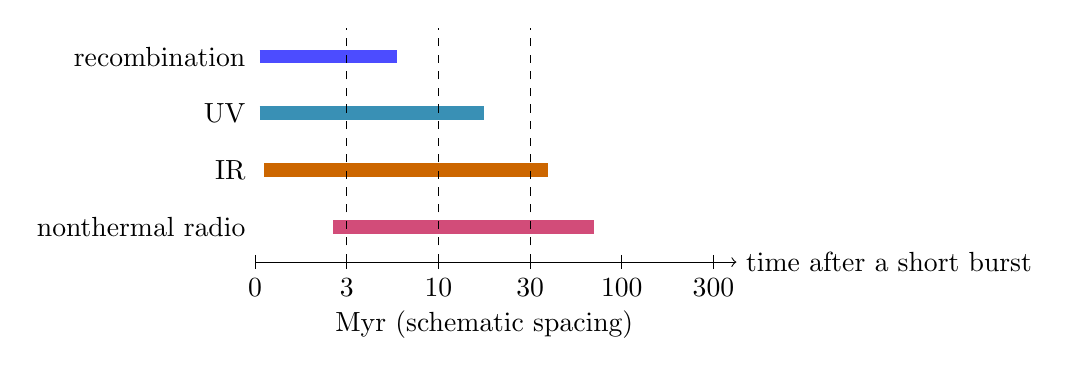
\begin{tikzpicture}[x=0.048\linewidth,y=0.9cm]
 \draw[->] (0,0)--(10.5,0) node[right] {time after a short burst};
 \foreach \x/\lab in {0/0,2/3,4/10,6/30,8/100,10/300}
   {\draw (\x,0.1)--(\x,-0.1) node[below] {\lab};}
 \node[below] at (5,-0.55) {Myr (schematic spacing)};
 \draw[line width=5pt,blue!70] (0.1,2.9)--(3.1,2.9);
 \node[left] at (0,2.9) {recombination};
 \draw[line width=5pt,cyan!70!black] (0.1,2.1)--(5.0,2.1);
 \node[left] at (0,2.1) {UV};
 \draw[line width=5pt,orange!80!black] (0.2,1.3)--(6.4,1.3);
 \node[left] at (0,1.3) {IR};
 \draw[line width=5pt,purple!70] (1.7,0.5)--(7.4,0.5);
 \node[left] at (0,0.5) {nonthermal radio};
 \draw[dashed] (2,0)--(2,3.3); \draw[dashed] (4,0)--(4,3.3);
 \draw[dashed] (6,0)--(6,3.3);
\end{tikzpicture}
\caption{Original qualitative response-window concept.  Bars indicate relative
sensitivity after a short stellar burst, not universal top-hat lifetimes.  Actual
kernels depend on metallicity, IMF, binaries, dust, and observing band.}
\label{fig:sfr-response-windows}
\end{figure}

\subsection{Stochastic populations and small apertures}

Standard calibrations assume that the stellar IMF and evolutionary phases are
adequately sampled.  In a small region or low-SFR galaxy, the number of ionizing stars
may be small.  H$\alpha$ luminosity then fluctuates strongly at fixed longer-timescale
SFR and can be zero between massive-star births.  This is a probability-distribution
problem, not necessarily evidence that the IMF has a different upper cutoff.

Spatial drift also matters.  Molecular gas, embedded infrared sources, exposed H\,II
regions, and young clusters are separated in both time and position.  On sufficiently
small apertures, gas and SFR tracers sample different evolutionary stages and the
depletion time scatters dramatically.  Galaxy-scale averages combine many regions and
recover more stable relations.

\section{Gas--star formation scaling relations}

Surface densities are often related by
\begin{equation}
 \Sigma_{\rm SFR}=A\left(\frac{\Sigma_{\rm gas}}{
 \Sigma_0}\right)^N
 \label{eq:kennicutt-schmidt}
\end{equation}
or expressed through a depletion time
\begin{equation}
 t_{\rm dep}=\frac{M_{\rm gas}}{\dot M_\star}.
 \label{eq:depletion-time}
\end{equation}
The slope $N$ depends on gas phase, dynamic range, spatial scale, regression method,
conversion factors, nondetections, and shared distance or inclination terms.  A
correlation does not identify the rate-limiting physics by itself.

Relations between HCN-like luminosity and star formation are sometimes interpreted as
evidence that a fixed-density gas component forms stars with constant efficiency.
However, line luminosity depends on excitation, opacity, abundance, and the entire
density probability distribution.  A linear relation can emerge from several models.
Multiple transitions, resolved density constraints, and independent masses are needed
to distinguish them.

\section{Spatially resolved evolutionary sequencing}

An idealized region passes from gas concentration to embedded sources, exposed H\,II
region, and feedback-cleared stellar association.  Observed maps contain many regions
at different phases.  Cross-correlating gas peaks and young-star peaks as a function
of aperture can constrain relative phase durations and separation scales, but only
under assumptions about region independence, steady formation rate, detectability,
and tracer lifetimes.

Line ratios add physical context to the sequence:
\begin{itemize}
 \item dense molecular tracers and deuterated species probe cold pre-stellar gas;
 \item warm H$_2$, high-$J$ CO, and complex molecules identify heating and shocks;
 \item radio recombination and free--free emission reveal deeply embedded massive
stars;
 \item optical recombination and forbidden lines map exposed ionized gas;
 \item broad molecular, optical, and X-ray features trace feedback and dispersal.
\end{itemize}
Selection by one stage biases inferred lifetimes of another.  A complete sequence
requires a parent sample defined independently of the tracers being timed.

\section{Inference checklist for a star-formation measurement}

Before turning a line luminosity into a rate or efficiency, record:
\begin{enumerate}
 \item the aperture and whether gas and stellar tracers are resolution matched;
 \item the assumed distance, attenuation, IMF, metallicity, and stellar models;
 \item the response timescale and whether steady star formation is plausible;
 \item contamination from AGN, shocks, diffuse ionized gas, evolved stars, or cirrus;
 \item photon escape and absorption by dust inside ionized regions;
 \item molecular excitation, abundance, opacity, and conversion-factor assumptions;
 \item stochastic population effects and treatment of nondetections;
 \item whether a quoted efficiency uses a mean-density, dense-gas, orbital, or other
 characteristic time.
\end{enumerate}
A star-formation tracer is best viewed as a calibrated temporal and spatial filter.
Its limitations become opportunities when several filters are modeled together.
